\chapter{代码重构} % Introduction chapter suppressed from the table of contents

重构代码的主要目的是使代码更容易维护,其他人更容易读懂。SOLID
原则是做好面向对象设计的基石,
例如随便搜索下面SOLID表格的关键字,可以找到很多参考资料。(SOLID
是取下面5原则的首英文字母)

%Screenshotfrom2022-12-2822-14-39.png

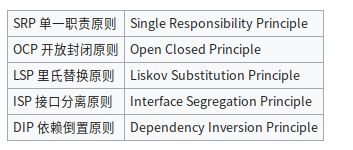
\includegraphics[width=10cm]{Screenshotfrom2022-12-2822-14-39.png}

也有很多参考书,如Gamma , Fowler 的经典书,Design Patterns
里面有对每一种设计模式的介绍与详细例子。

\hypertarget{ux5982ux4f55ux5b66ux597dsolidux6253ux597dux57faux7840ux505aux91cdux6784}{%
\subsection{如何学好SOLID,打好基础做重构}\label{ux5982ux4f55ux5b66ux597dsolidux6253ux597dux57faux7840ux505aux91cdux6784}}

培训经验:以前我们传统教学方式做重构设计模式培训,分别解释、举例说明二十几个设计模式,学生听完后,很快就忘记了,没有任何效果。\\
要有效学习,程序员必须积极动脑动手,不能单靠理论课。从Weinberg先生教程序员的例子(详见附件)看到,如果先在讲课时强调某些重点,然后配上编程练习,学员才能真正吸收,后面能在项目中用上。

\hypertarget{ux5982ux4f55ux63d0ux5347ux5b66ux5458ux7684ux5174ux8da3ux4e0eux52a8ux529b}{%
\subsection{如何提升学员的兴趣与动力}\label{ux5982ux4f55ux63d0ux5347ux5b66ux5458ux7684ux5174ux8da3ux4e0eux52a8ux529b}}

我们后面改用工作坊的培训方式,减少理论讲诉,要求学生在电脑写小程序,效果比本来仅仅是讲的好。有些领悟能力比较强的学生,都可以很好完成一系列的练习题,但还是有百分之四、五十跟不上。我们在想问题在哪里?如何可以改善?\\
我们回顾一下问题在哪里?跟得上的学生本身领会力就比较强,软件开发的基础也较好,所以可以很容易跟得上我们设置的编程练习,在课堂上就可以按我们的设计完成大部分的编程练习。问题出在那些比较弱的学员,本身对编程和面向对象一知半解,开始时候觉得写小程序跟不上那些其他高水平的同学,后面就放弃了。\\
培训新入职员工也面临类似问题,而且如果未能在头几个月把重点学好,养成习惯,后面便难以改正。\\
七八十年代,麻省理工科学家Parpert先生,他本来一直研究人工智能,他发现很多美国小学生都跟不上学校的数学与几何课,根因是老师用传统教学方法,学生没有兴趣学,他后面就利用乌龟几何(Mindstorm)做实验,让小学生可以轻轻松松用电脑编程、玩游戏学习几何。(详见附件)

所以后面我们就利用乌龟学数学的思路,设计了一系列的基于设计模式的练习题。设计模式最大的好处就是方便后面需求的更新。所以我们把那些常用的设计模式写成模块,就像乐高积木一样,让学员可以调用,然后学生就可以像乐高积木,尽量利用那些设计模式的组件,针对课题目设计程序。\\
做了完了第一段后,就有些改变 -
新增或者减少需求,教他们怎么可以再利用设计模式更新程序,达到题目的要求。我发现这种方式的话,学生后面在实际工作中就更能用上设计模式,因为与之前单纯对应题目编程不同,学员有更大空间设计总体的架构与功能,与前面提的美国小学生一样,因有兴趣,便能很快学到面向对象的编码原理。\\

\hypertarget{ux4ec0ux4e48ux65f6ux5019ux505aux91cdux6784}{%
\subsection{什么时候做重构}\label{ux4ec0ux4e48ux65f6ux5019ux505aux91cdux6784}}

写程序与写文章类似,都是一个逐步优化的过程,初稿可能先写一些重点,里面的细节需要不断的评审、优化,就更不用说语法、错别字了。\\
%\href{文件:环形图1.jpg}{500px}

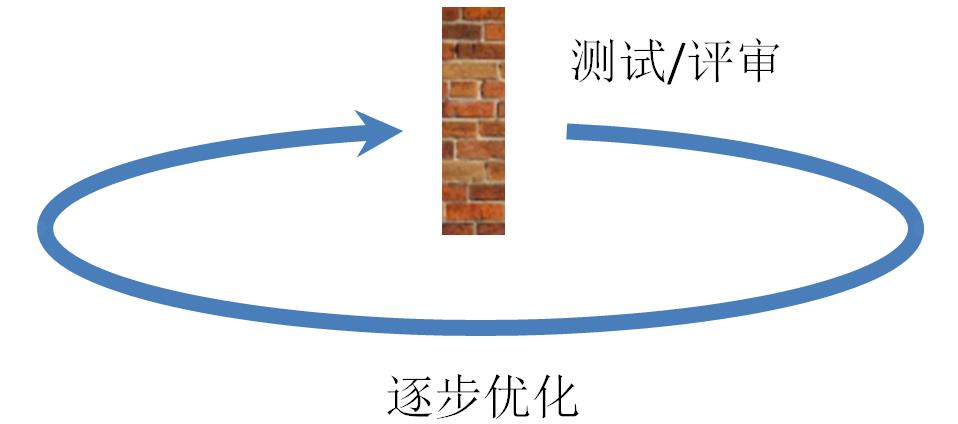
\includegraphics[width=10cm]{环形图1.jpg}

虽然现在我写程序的时间不多,但还是依据同样思路。先把程序写出来,基于测试驱动开发的原则,通过单元测试,但通常第一版程序有很多不足,比如不能达到SOLID等面向对象要求,所以会依据设计模式原则优化代码,并利用自动化单元测确保每次改动后程序可以跑通,所以写代码也是逐步优化的过程,只是代码错了一点就会跑不通,文章因为容错性强,错个别字不影响读者读懂。所以专业软件工程师不会等到维才的程度才去重构,而是持续的小重构,一直考虑软件的维护性、扩展性,如果达不到质量水平,宁可不发布,好比具备专业手艺的陶瓷工匠会砸碎不达标的陶器;或作曲家宁愿烧毁自己不满意的作品,不发布一样。

\framebox{%
\begin{minipage}[t]{0.97\columnwidth}\raggedright
出书和单独分享文章不一样,要注意整体的架构,不然后面就组合不起来。下面是我的经验教训:
我一直都接触客户,收集了很多相关实例,加上参考国外的最佳实践写成分享文章,在公众号发布,也会在微信群朋友圈里面请大家评审、完善。原本是不知道如何开始,后面有了经验越来越懂如何集合客户现场听到的故事,与书本上的知识,写成分享文章。朋友圈里有朋友提议我出版书,但是在出版前要先发书的目录架构和章节内容给总编辑审批。我就充满信心,觉得之前写过的分享文章都适用,写了目录再抽部分以前分享的文章,然后对朋友说``这本书的内容起码完成了7成,剩下部分再用两三个月就可以写完并出版了。''

朋友听到很开心,就联系出版社,让我发目录和两个前面的章节给编辑。
我满以为问题不大,过了两天朋友问总编,得到简单回应:``文章都很散,距离出版很远。''

我立马感到当头棒喝,重新回看以往的分享文章,它们作为散文没问题,但是有很多跟书的主线无关
-
比如觉得有兴趣就谈谈香港70年代的成功要素,另外也加一些名人的成功经历等。导致绝大部分的文章都要重新写,我构思书的总体架构,改成小手册形式,再把以前的长篇分享改写成不超过4页的小章节,导致接近一个人月的返工。

一本小手册不到20万字,因开始时没有注意总体架构,导致大量返工。如果是几十万行甚至一两百万行代码的软件系统,可以想象等到后面需要重构是多困难。\strut
\end{minipage}}

\hypertarget{ux4ee3ux7801ux89c4ux8303}{%
\subsection{代码规范}\label{ux4ee3ux7801ux89c4ux8303}}

制定编码标准是其中一条XP实践,因为若要写好程序、减少错误,必须预先把常见问题罗列出来,提醒大家。\\
客户:我们一直没有,可否直接参考其他公司的标准?\\
我:某公司想快速通过认证,但公司一直都没有自己的标准过程,顾问说:``不担心,我们可以提供其他已通过认证公司的过程''你觉得公司最终会有质量改善吗?\\
客户:应该没有,因过程不是从本身实战经验出来,对团队提升质量没有用。\\
我:非常赞同,所以编码标准也必须归纳自己动手的实战经验,像刚才乌龟几何一样,让学生自己经历过解决问题,有及时的反馈,他才能真正学会。编码规范很重要,但规范不应从人家那里复制过来,而是从自己常见的问题总结出来,对团队才有意义。\\

\hypertarget{ux6301ux7eedux96c6ux6210}{%
\subsection{持续集成}\label{ux6301ux7eedux96c6ux6210}}

文章、书本等文字性的不像代码、软件,错一个字都会导致跑不通的问题。所以几十年前人们无法想象现在可以做到这么大型的软件系统开发都起码要几个月,系统规模也不会太大。现代软件开发有很多辅助工具,可以一边写一边检测,也有各个层次的测试来确保软件没问题,并能自动化,让团队可用每天发布,也能支持大型分布式系统。
下一章节,我们看看如何利用自动化工具帮我们做到持续集成、持续发布。

\hypertarget{ux9644ux4ef6}{%
\section{附件}\label{ux9644ux4ef6}}

\hypertarget{a1-ux5c0fux5b69ux5229ux7528ux4e4cux9f9fux73a9ux51e0ux4f55ux6e38ux620fturtle-geometryux4f8bux5b50}{%
\subsection{小孩利用乌龟玩几何游戏(Turtle
Geometry)例子}\label{a1-ux5c0fux5b69ux5229ux7528ux4e4cux9f9fux73a9ux51e0ux4f55ux6e38ux620fturtle-geometryux4f8bux5b50}}

美国传统怎么教小学生学数学、几何。但是传统用纸和笔的方法,小学生就没有兴趣学,导致跟不上。原因很简单,我们以数学为例,现在很多小学生学数学,还是我们几十年前那种,背九宫表算乘除。以前我们的年代没有计算机,电脑就更不用说了,所以逼着人要背那些表,就跟古代学习用算盘计算一样。但现在计算机已经可以随时买到,且很便宜,手机也有计算功能,所以他们就认为这种传统的学习数学方式已经无用,几何也一样。如果学生比较擅长数学还好,但假如有跟不上的,就觉得会觉得自己不是学数学的这块料,后面就放弃了数学。\\
于是Parpert先生教小孩利用乌龟玩几何游戏(Turtle Geometry):

%\href{文件:mindstorm_p5.jpg}{文件:mindstorm p5.jpg}\\

\includegraphics[width=10cm]{mindstorm_p5.jpg}
学生可以简单利用往前往右往左的命令,画出正方形、三角形:

%\href{文件:mindstorm_p70.jpg}{文件:mindstorm p70.jpg}\\
%\href{文件:mindstorm_p71.jpg}{文件:mindstorm p71.jpg}\\

%\includegraphics[width=10cm]{mindstorm_p70.jpg}\\
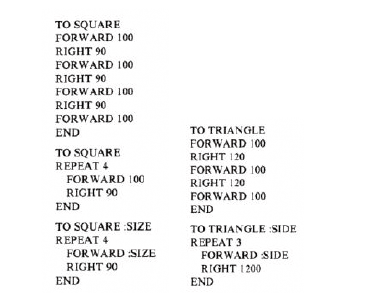
\includegraphics[width=6cm]{微信截图_20230323093342.png}\\
编码有误,学生自己调代码,把三角形的方向改正,才能画成一间屋:

%\href{文件:mindstorm_p72.1.jpg}{文件:mindstorm p72.1.jpg}\\
%\href{文件:mindstorm_p72.2.jpg}{文件:mindstorm p72.2.jpg}\\
%\href{文件:mindstorm_p73.jpg}{文件:mindstorm p73.jpg}\\


%\includegraphics[width=10cm]{mindstorm_p721.jpg}\\
%\includegraphics[width=10cm]{mindstorm_p722.jpg}\\
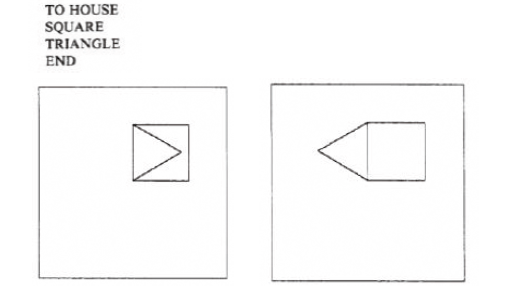
\includegraphics[width=6cm]{微信截图_20230323093355.png}\\
甚至圆形,在这个基础上,他们可以继续画一朵花,通过这个方式,学生就觉得自己可以掌握。

%\href{文件:mindstorm_p95.1.jpg}{文件:mindstorm p95.1.jpg}\\
%\href{文件:mindstorm_p95.2.jpg}{文件:mindstorm p95.2.jpg}\\
%\href{文件:mindstorm_p96.jpg}{文件:mindstorm p96.jpg}\\
%\href{文件:mindstorm_p97.jpg}{文件:mindstorm p97.jpg}\\

\includegraphics[width=10cm]{mindstorm_p951.jpg}\\
\includegraphics[width=10cm]{mindstorm_p952.jpg}\\
\includegraphics[width=10cm]{mindstorm_p96.jpg}\\
\includegraphics[width=10cm]{mindstorm_p97.jpg}\\


\hypertarget{a2ux6e29ux4f2fux683cux7684ux6559ux5b66ux5b9eux9a8c}{%
\subsection{温伯格的教学实验}\label{a2ux6e29ux4f2fux683cux7684ux6559ux5b66ux5b9eux9a8c}}

伯格先生在60年代教程序员,就发现很多人没有动手,导致上课学过的东西无法用在工作上。为了解决这个问题,他在教IBMOS360时,把本来的理论课改成一些工作坊教学形式。他还做了一个小实验,在一班讲课的时候强调要注意一些OS语言的常见问题,例如如何避免错误的空格导致编程失败,他发现平均下来还是有83\%的错误。而另外一个课堂上没有强调这些细节的班级的错误是87\%。他还做了另外一个实验,对第二个班学生增加越来越难的练习题。到了第10题,10个练习,17个学生中有13个基本上就掌握了这技巧,没有再犯同样错误。从这两个实验可以看到,要有效学习,程序员必须积极动脑动手,不能单靠理论课。

\hypertarget{references}{%
\section{References}\label{references}}

1. Parpert, Seymour: \textbf{\emph{Mindstorms: children, computers, and
powerful ideas}} Basic Books, 1980.\\
2. Weinberg, Gerald: '''''The Psychology of Computer Programming: Silver
anniversary edition '''''2021(1971)\\




